\chapter{The GeoJSON Export Extension}\label{ch:the-geojson-export-extension}
\section{Overview}
The \textbf{GeoJSON Export} extension is an extension build using the OpenRefine extension architecture and its
purpose is provide the OpenRefine user with the functionality of exporting geospatial data (in an OpenRefine project) to
the GeoJSON (.geojson) format.\\
\newline
The extension supports lat/lon values and WKT strings.
\section{The GeoJSON Export format}
GeoJSON is a format for encoding a variety of geographic data structures.
It is a format designed for representing \textit{Simple Features} and their attributes.
It is based on the JSON format.\\
\newline
GeoJSON supports the following geometry types:
\mintinline[breaklines]{bash}{Point, LineString, Polygon,MultiPoint, MultiLineString}
and \mintinline[breaklines]{bash}{MultiPolygon}.
Geometric objects with additional properties are \mintinline{bash}{Feature} objects.
Sets of features are contained by \mintinline{bash}{FeatureCollection} objects. \cite{WhatIsGeoJSON}\\
\newline

A \textit{.geojson} file looks something like this:
\begin{minted}[breaklines, linenos]{json}
{
  "type": "FeatureCollection",
  "features": [
    { "type": "Feature",
      "geometry": {"type": "Point", "coordinates": [102.0, 0.5]},
      "properties": {"prop0": "value0"}
      },
    { "type": "Feature",
      "geometry": {
        "type": "LineString",
        "coordinates": [
          [102.0, 0.0], [103.0, 1.0], [104.0, 0.0], [105.0, 1.0]
          ]
        },
      "properties": {
        "prop0": "value0",
        "prop1": 0.0
        }
      },
    { "type": "Feature",
       "geometry": {
         "type": "Polygon",
         "coordinates": [
           [ [100.0, 0.0], [101.0, 0.0], [101.0, 1.0],
             [100.0, 1.0], [100.0, 0.0] ]
           ]

       },
       "properties": {
         "prop0": "value0",
         "prop1": {"this": "that"}
         }
       }
    ]
}
\end{minted}
More information on the \textit{.geojson} file extension can be found here: \href{https://geojson.org/}{https://geojson.org/}
\pagebreak
\section{Architecture and Design}
\subsection{Architecture}
The extension is built using the \href{https://www.java.com/en/}{Java} programming language (Java Platform SE 8),
which is fully compliant with the OpenRefine development environment.
The extension is built as a "separate" component from OpenRefine, meaning it has to manually be added/installed to an
existing OpenRefine application environment.\\
\newline
The extension is compiled using \href{https://maven.apache.org/index.html}{Apache Maven} and consists of client-side
resources such as .html, .css, .less, .js files and of server-side resources i.e. Java classes. These Java classes are
bundled during the initialization of OpenRefine and can consist of controllers, commands, functions etc. They are invoked
using HTTP requests such as GET or POST with AJAX. All of the necessary client-side resources and server-side resources must be
injected to OpenRefine using the \mintinline{java}{init()} function of the extension.\\
\newline
When the extension is built, all of the Java classes and the client-side resources are stored in a directory which need to be copied to
the OpenRefine installation \\extension directory in order for it to be bundled together with the OpenRefine application.\\
\newline
An extension of OpenRefine has the following file structure:
\begin{minted}
[
    frame=lines
]
{bash}
pom.xml
  src/
      com/foo/bar/... *.java source files
  module/
      *.html, *.vt files
      scripts/... *.js files
      styles/... *.css and *.less files
      images/... image files
      MOD-INF/
          lib/*.jar files
          classes/... java class files
          module.properties
          controller.js
\end{minted}
More information on installing extensions can be found \href{https://docs.openrefine.org/manual/installing#installing-extensions}{here}.
OpenRefine's official documentation also includes an article on how to write extensions \href{https://docs.openrefine.org/technical-reference/writing-extensions}{here}.\\
\newline
\subsection{Design Decisions}
\begin{table}
    \begin{tabularx}{\textwidth}{| X | X |}
        \hline
        \textbf{Decision} & \textbf{Reason}\\[1cm]
        \hline
        The \href{https://github.com/bjornharrtell/jts2geojson}{jts2geojson} library is used for
        converting JTS geometry to GeoJSON. & The \href{https://github.com/bjornharrtell/jts2geojson}{jts2geojson} library is
        able to convert JTS geometries to GeoJSON and back. \\
        \hline
        The \href{https://github.com/locationtech/jts}{JTS Topology Suite} library is used to process the geometry objects. &
        The \href{https://github.com/bjornharrtell/jts2geojson}{jts2geojson} requires JTS Geometry in order to be able to convert it to GeoJSON.
        The latitude/longitude columns and WKT strings are used together with the JTS library to create JTS Geometry.
        Points are created using their X and Y values into a JTS Point Geometry and WKT strings are converted to JTS geometry
        using the \href{https://locationtech.github.io/jts/javadoc/org/locationtech/jts/io/WKTReader.html}{\mintinline{bash}{WKT Reader}}
        JTS class. These geometries are then continously stored as GeoJSON features and at the end of the iteration,
        they are added to the \mintinline{bash}{FeatureCollection}.
        This \mintinline{bash}{FeatureCollection} is used as GeoJSON data for the exported GeoJSON file.\\
        \hline
        The Well-Known Text (WKT) geometry is used as the geometry representation format for exporting to GeoJSON. &
        Any type of geometry object can be represented using WKT and it can be stored in a single
        cell without having any dependencies to another cell or needing more than one cell.\\
        \hline
    \end{tabularx}
    \caption{Design Decisions - GeoJSON Export}
\end{table}
\subsubsection{The Solution Stack}
This extension was built using the Java programming language, version 8, for the back end. For the front-end portion,
a combination of Javascript, the jQuery library, LESS and HTML was used. \\
\newline
\href{https://www.java.com/en/}{Java} is a powerful general-purpose programming language.
It is used to develop desktop and mobile applications,
big data processing, embedded systems, and so on.
According to Oracle, the company that owns Java, Java runs on 3 billion devices worldwide, which makes Java one of the most popular programming languages. cite{WhatIsJava}\\
\newline
The reason why this plugin was chosen to be built and developed using Java is
because of OpenRefine, it is programmed using Java,
so all its extensions must also be written in Java (using OpenRefine\'s extension
architecture). All of the OpenRefine extensions are developed inside the
OpenRefine environment as a separate bundled directory and must use OpenRefine\'s
native Java methods in order to be communicate with OpenRefine\'s core engine.\\
It is also an Object-Oriented programming language, which runs under any operating system
(because of its compiler) and uses inheritance and abstract methods (Object Oriented programming principles),
which turned out to be useful and appropriate for the nature of this extension.\\
\newline

For the front-end, the usual front-end stack was used to develop the UI parts i.e. Javascript, jQuery, LESS and HTML.
\pagebreak=
\section{Implementation}
\subsection{Overview}
The extension adds a new export option to OpenRefine which allows the OpenRefine users to
export their data to the \textit{GeoJSON} format. The export option is called \textit{GeoJSON (.geojson)...} and the ellipsis
indicates that there is a dialog for confiruing the export options before successfully exporting the data.
\subsection{Exporting the data}
This extension expects some type of geospatial data in the OpenRefine project.
It recognizes columns containing latitude/longitude values (X and Y) and columns containing WKT strings (of any Geometry).\\
\newline
The user can open the export dialog by clicking on the \textit{Export} drop-down button of the OpenRefine project and then clicking
on the \textit{GeoJSON (.geojson)...} button.
This will open up a dialog where the user has to specify the geometry columns and also the columns that they want to
include as properties for the GeoJSON features.\\
\newline

\begin{figure}[H]
    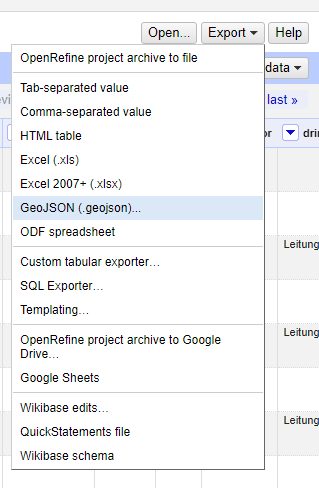
\includegraphics[width=7cm]{./Figures/GeoJSON_Export/geojson_export_button}
    \caption{The GeoJSON export button, located on the top right of an OpenRefine project}
\end{figure}

The dialog lets the user choose the name of the \textit{.geojson} file, the latitude/longitude columns, the WKT column
and the columns they want to include as properties of the geometry features. Latitude, longitude or WKT columns can be
ommitted from the export if such columns do not exist, however, if latitude or longitude columns are selected,
both of the columns are needed for a successful export (latitude and longitude).\\
\newline
The right side of the dialog lets the user choose what columns they want to include as properties to each of the GeoJSON features,
with the geometry columns selected on the left being ommitted from the properties table.\\
\newline
The user can also select the numeric scale of the decimal values of the geometries by tweaking the \textbf{Geometry numeric scale}
option at the bottom of the dialog to a different number, the default value is \textbf{7}. This number represents the
number of decimal digits to the right  of the decimal point of a decimal number, e.g. \textit{47.4955184} has a numeric scale of
7 because there are 7 numbers to the right of the decimal point of the number (this being the default numeric scale).
This numeric scale is used while processing lat/lon values or WKT values. \\
\newline
More information on what a numeric scale is can be found here:
\href{https://docs.microsoft.com/en-us/sql/t-sql/data-types/precision-scale-and-length-transact-sql?view=sql-server-ver15}{https://docs.microsoft.com/en-us/sql/t-sql/data-types/precision-scale-and-length-transact-sql?view=sql-server-ver15}.

\begin{figure}[H]
    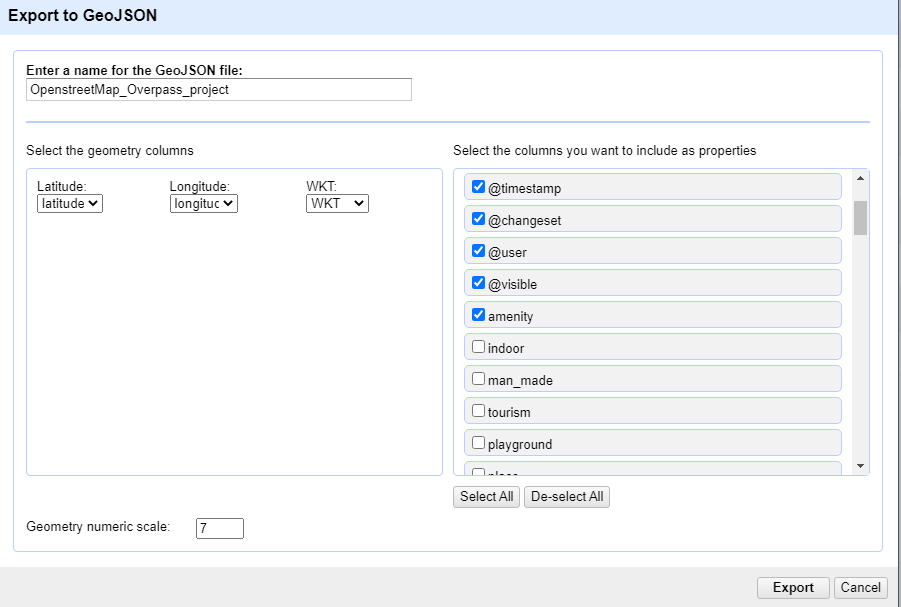
\includegraphics[width=\linewidth]{./Figures/GeoJSON_Export/geojson_export_dialog}
    \caption{The GeoJSON export dialog}
\end{figure}

\subsection{The Conversion Process}
For converting the geospatial data to GeoJSON, the \href{https://github.com/bjornharrtell/jts2geojson}{jts2geojson} Java library was used. This library converts
JTS geometries to GeoJSON (and vice-versa). It internally uses the JTS library to create the geometries and then utilizes those geometries to create GeoJSOn
features out of.\\
\newline
A GeoJSON \mintinline{bash}{FeatureCollection} is first created with empty \mintinline{bash}{Features}. The Features are then dynamically added to the feature collection by
iterating through the OpenRefine rows. The extension supports all types of Features, including:
\begin{itemize}
    \item Points
    \item LineStrings
    \item Polygons
    \item MultiPoints
    \item MultiLineStrings and
    \item MultiPolygons
\end{itemize}
If only the latitude and longitude columns were selected, then the extension reads those values and creates simple Points out of them. These points are then created as Features
and included in the GeoJSON file, along with their properties, as selected on the export dialog.\\
\newline
Here's an example of an exported GeoJSON data (with only a few Features):
\begin{minted}[tabsize=2, breaklines, linenos]{json}
{
  "type" : "FeatureCollection",
  "features" : [ {
    "type" : "Feature",
    "geometry" : {
      "type" : "Point",
      "coordinates" : [ 8.718769, 47.350209 ]
    },
    "properties" : {
      "amenity" : "drinking_water",
      "@id" : "8899069808"
    }
  }, {
    "type" : "Feature",
    "geometry" : {
      "type" : "Point",
      "coordinates" : [ 8.603137, 47.536676 ]
    },
    "properties" : {
      "amenity" : "drinking_water",
      "@id" : "2091396746"
    }
  }, {
    "type" : "Feature",
    "geometry" : {
      "type" : "Point",
      "coordinates" : [ 8.58352, 47.358378 ]
    },
    "properties" : {
      "amenity" : "drinking_water",
      "@id" : "698059005",
      "operator" : "WVZ"
    }
  }]
}
\end{minted}
Here is also the code that e.g. converts a Point WKT to a Point Features in GeoJSON:
\begin{minted}[tabsize=2, breaklines, linenos]{java}
    org.wololo.geojson.Point point = (org.wololo.geojson.Point) geometry;
    double[] coordinates = point.getCoordinates();
    double[] _coordinates = new double[]{
            Math.round(coordinates[0] * scaleFactor) / scaleFactor,
            Math.round(coordinates[1] * scaleFactor) / scaleFactor
    };

    org.wololo.geojson.Point _point = new org.wololo.geojson.Point(_coordinates);

    features.add(new Feature(_point, properties));
\end{minted}
The scale factor corresponds to the numeric scale specified in the export dialog i.e. 10 in the power of the \textit{geometry numeric scale}.\\
\newline
At the end of the rows, all the features are added to the \mintinline{bash}{FeatureCollection} object and written to the GeoJSON file.
\subsection{Testing}
This extension includes some unit testing. The framework used for unit testing is the \href{https://testng.org/}{TestNG} framework.
\subsection{Unit Testing}
TestNG is a testing framework inspired from JUnit and NUnit. It is designed to cover all categories of testing.\\
This extension contains minimal unit testing for some of its important functions and everytime the CI/CD pipeline is run in GitLab, the
extension's unit tests are executed to see if everything is still working as expected.
\pagebreak
\section{Usage \& Examples}
\subsection{Usage}
\begin{enumerate}
    \item Launch OpenRefine with the \textbf{GeoJSON Export} extension
    \item Create a new project or open an existing one
    \item Make sure there are atleast latitude/longitude columns or a WKT column consisting the data that needs to be exported to GeoJSON
    \item Under the \textit{Export} drop-down, click on the \textit{GeoJSON (.geojson)...} option
    \item In the export dialog, choose the latitude/longitude columns or the WKT column (or all of them)
    \item Choose the columns that need to be included as properties to each of the GeoJSON features inside the FeatureCollection
    \item Override the geometry numeric scale if necessary.
    \item Choose a name for the \textit{.geojson} file and click on the \textit{Export} button at the bottom of the dialog
\end{enumerate}
\subsection{Examples}
Here are some examples of GeoJSON exported data from OpenRefine using this extension:
\begin{minted}[tabsize=2, breaklines, linenos]{json}
{
  "type" : "FeatureCollection",
  "features" : [ {
    "type" : "Feature",
    "geometry" : {
      "type" : "Point",
      "coordinates" : [ 8.5740834, 47.556292 ]
    },
    "properties" : {
      "end_date" : "mid C14",
      "historic:civilization" : "medieval",
      "historic" : "castle",
      "access" : "yes",
      "point_delimited" : "47.556292;8.574083",
      "description" : "Nordöstlich über Teufen markanter, allseits steil abfallender Burghügel mit schwachen Mauerresten eines Turmes und der Umfassungsmauer. Sitz der Freiherren v. Teufen, erwiesen 1285. 1334 zerstört. (Quelle: Burgenverein.ch)",
      "name:gsw" : "Hohen-Tüfen",
      "ruins" : "yes",
      "castle_type" : "defensive",
      "name" : "Burgstelle Hohenteufen",
      "@id" : "1862065036",
      "wikipedia" : "de:Burgstelle Hohenteufen",
      "wikidata" : "Q29932628",
      "ele" : "568",
      "start_date" : "late C13"
    }
  }, {
    "type" : "Feature",
    "geometry" : {
      "type" : "Point",
      "coordinates" : [ 7.0567095, 47.3659388 ]
    },
    "properties" : {
      "name:de" : "Schloss Montvoie",
      "historic" : "castle",
      "point_delimited" : "47.365939;7.056710",
      "ruins" : "yes",
      "castle_type" : "stately",
      "name" : "Château de Montvoie",
      "name:en" : "Montvoie Castle",
      "@id" : "1521546163",
      "wikidata" : "Q6906665"
    }
  } ]
}
\end{minted}
This GeoJSON document contains two Features of type \mintinline{bash}{Point}, their coordinates and some non-spatial properties that
were extracted from OpenStreetMap.
\begin{minted}[tabsize=2, breaklines, linenos]{json}
{
  "type" : "FeatureCollection",
  "features" : [ {
    "type" : "Feature",
    "geometry" : {
      "type" : "LineString",
      "coordinates" : [ [ 7.7529493, 47.3816381 ], [ 7.7529443, 47.3816044 ] ]
    },
    "properties" : {
      "historic" : "castle_wall",
      "ruins" : "castle"
    }
  }, {
    "type" : "Feature",
    "geometry" : {
      "type" : "MultiPolygon",
      "coordinates" : [ [ [ [ 8.1404353, 46.1959036 ], [ 8.1404352, 46.195953 ], [ 8.1402542, 46.195952 ], [ 8.1401752, 46.1959494 ], [ 8.140174, 46.1958587 ], [ 8.140173, 46.1957775 ], [ 8.1404439, 46.1957792 ], [ 8.1404431, 46.1958362 ], [ 8.1403847, 46.1958358 ], [ 8.1403838, 46.1959033 ], [ 8.1404353, 46.1959036 ] ] ], [ [ [ 8.1404353, 46.1959036 ], [ 8.1404918, 46.195904 ], [ 8.1404928, 46.1958365 ], [ 8.1404731, 46.1958364 ], [ 8.1404431, 46.1958362 ], [ 8.1404353, 46.1958362 ], [ 8.1403847, 46.1958358 ], [ 8.1403838, 46.1959033 ], [ 8.1404353, 46.1959036 ] ] ] ]
    },
    "properties" : {
      "addr:housename" : "Stockalperturm",
      "historic" : "castle",
      "building:levels" : "5",
      "type" : "site",
      "addr:postcode" : "3907",
      "building" : "hotel",
      "addr:city" : "Gondo",
      "addr:housenumber" : "21",
      "material" : "stone",
      "castle_type" : "defensive",
      "name" : "Stockalperturm",
      "addr:street" : "Simplonstrasse",
      "wikidata" : "Q443634"
    }
  }, {
    "type" : "Feature",
    "geometry" : {
      "type" : "MultiPolygon",
      "coordinates" : [ [ [ [ 6.8898688, 46.4696051 ], [ 6.8899728, 46.4696341 ], [ 6.8899767, 46.4696179 ], [ 6.8901071, 46.4696706 ], [ 6.890114, 46.4696591 ], [ 6.8902238, 46.4696794 ], [ 6.8902169, 46.4697111 ], [ 6.890367, 46.4697395 ], [ 6.8903758, 46.4697064 ], [ 6.8904591, 46.4697179 ], [ 6.8905003, 46.4695693 ], [ 6.8903934, 46.4695126 ], [ 6.8904191, 46.4694871 ], [ 6.8904434, 46.4694556 ], [ 6.8903476, 46.4694096 ], [ 6.8903023, 46.4694626 ], [ 6.890165, 46.4694052 ], [ 6.889967, 46.4693767 ], [ 6.889872, 46.4693709 ], [ 6.8898422, 46.4694431 ], [ 6.889793, 46.4695176 ], [ 6.8897694, 46.469509 ], [ 6.8897525, 46.4695302 ], [ 6.8897068, 46.469514 ], [ 6.8896702, 46.4695595 ], [ 6.8897096, 46.4695876 ], [ 6.8896953, 46.4696593 ], [ 6.889794, 46.4696821 ], [ 6.8898091, 46.469666 ], [ 6.8898688, 46.4696051 ] ], [ [ 6.8899697, 46.4695339 ], [ 6.8900081, 46.469478 ], [ 6.8901726, 46.4695437 ], [ 6.8901836, 46.4695256 ], [ 6.890302, 46.4695686 ], [ 6.8902779, 46.469617 ], [ 6.8899697, 46.4695339 ] ] ] ]
    },
    "properties" : {
      "historic" : "castle",
      "castle_type" : "defensive",
      "name" : "Château de Blonay",
      "wikipedia" : "fr:Château de Blonay",
      "type" : "multipolygon",
      "wikidata" : "Q684917"
    }
  } ]
}
\end{minted}
This GeoJSON document contains Features of type \mintinline{bash}{LineString} and \mintinline{bash}{MultiPolygon},
their coordinates and some non-spatial properties that were extracted from OpenStreetMap.
